\chapter{Pairings: temperature dependency} % Main chapter title

\label{Appendix.pairingtemperaturedependency} 
\fancyhead[LO, RE]{Part V. \emph{Appendices}}
\chead{G. \emph{Pairings: temperature dependency}}


%----------------------------------------------------------------------------------------
In this appendix we calculate the temperature dependency of the inter- and intrawire pairings. The expected behaviour can be inferred from the standard BCS-treatment, see e.g. \cite[p. 369]{PlischkeStatPhys}. From here we expect that the pairings have their maximal value for $T = 0$ and decreases monotonically until a critical temperature, $T_c$, is reached. It is however not entirely clear, what effect the presence of two pairings has on this behaviour. 

We have done the calculation for an interwire distance just above the critical distance, $d_c$. The result of the analysis is shown in figure \ref{fig.maximalpairingsTdepend_2wires}. Since we are above the critical distance, we expect the \textit{intra}wire pairing to be dominant. This is indeed the case for temperatures $T \approx 0$. However, we notice that the interwire pairing actually has a higher critical temperature, and in particular is dominant for $0.1 < T / T_F < 0.13$. Besides this, the overall expected behaviour is observed. We observe that the interwire pairing has a small downward kink, where the intrawire pairing vanishes. The same behaviour is seen when the intrawire pairing is dominant. This means, that the dominant pairing would be higher at low temperatures if the other pairing was not present: there is a trade off between the size of the individual pairings and the presence of a second pairing.

\begin{figure} 
\begin{center}  
% GNUPLOT: LaTeX picture with Postscript
\begingroup
  \makeatletter
  \providecommand\color[2][]{%
    \GenericError{(gnuplot) \space\space\space\@spaces}{%
      Package color not loaded in conjunction with
      terminal option `colourtext'%
    }{See the gnuplot documentation for explanation.%
    }{Either use 'blacktext' in gnuplot or load the package
      color.sty in LaTeX.}%
    \renewcommand\color[2][]{}%
  }%
  \providecommand\includegraphics[2][]{%
    \GenericError{(gnuplot) \space\space\space\@spaces}{%
      Package graphicx or graphics not loaded%
    }{See the gnuplot documentation for explanation.%
    }{The gnuplot epslatex terminal needs graphicx.sty or graphics.sty.}%
    \renewcommand\includegraphics[2][]{}%
  }%
  \providecommand\rotatebox[2]{#2}%
  \@ifundefined{ifGPcolor}{%
    \newif\ifGPcolor
    \GPcolorfalse
  }{}%
  \@ifundefined{ifGPblacktext}{%
    \newif\ifGPblacktext
    \GPblacktexttrue
  }{}%
  % define a \g@addto@macro without @ in the name:
  \let\gplgaddtomacro\g@addto@macro
  % define empty templates for all commands taking text:
  \gdef\gplbacktext{}%
  \gdef\gplfronttext{}%
  \makeatother
  \ifGPblacktext
    % no textcolor at all
    \def\colorrgb#1{}%
    \def\colorgray#1{}%
  \else
    % gray or color?
    \ifGPcolor
      \def\colorrgb#1{\color[rgb]{#1}}%
      \def\colorgray#1{\color[gray]{#1}}%
      \expandafter\def\csname LTw\endcsname{\color{white}}%
      \expandafter\def\csname LTb\endcsname{\color{black}}%
      \expandafter\def\csname LTa\endcsname{\color{black}}%
      \expandafter\def\csname LT0\endcsname{\color[rgb]{1,0,0}}%
      \expandafter\def\csname LT1\endcsname{\color[rgb]{0,1,0}}%
      \expandafter\def\csname LT2\endcsname{\color[rgb]{0,0,1}}%
      \expandafter\def\csname LT3\endcsname{\color[rgb]{1,0,1}}%
      \expandafter\def\csname LT4\endcsname{\color[rgb]{0,1,1}}%
      \expandafter\def\csname LT5\endcsname{\color[rgb]{1,1,0}}%
      \expandafter\def\csname LT6\endcsname{\color[rgb]{0,0,0}}%
      \expandafter\def\csname LT7\endcsname{\color[rgb]{1,0.3,0}}%
      \expandafter\def\csname LT8\endcsname{\color[rgb]{0.5,0.5,0.5}}%
    \else
      % gray
      \def\colorrgb#1{\color{black}}%
      \def\colorgray#1{\color[gray]{#1}}%
      \expandafter\def\csname LTw\endcsname{\color{white}}%
      \expandafter\def\csname LTb\endcsname{\color{black}}%
      \expandafter\def\csname LTa\endcsname{\color{black}}%
      \expandafter\def\csname LT0\endcsname{\color{black}}%
      \expandafter\def\csname LT1\endcsname{\color{black}}%
      \expandafter\def\csname LT2\endcsname{\color{black}}%
      \expandafter\def\csname LT3\endcsname{\color{black}}%
      \expandafter\def\csname LT4\endcsname{\color{black}}%
      \expandafter\def\csname LT5\endcsname{\color{black}}%
      \expandafter\def\csname LT6\endcsname{\color{black}}%
      \expandafter\def\csname LT7\endcsname{\color{black}}%
      \expandafter\def\csname LT8\endcsname{\color{black}}%
    \fi
  \fi
    \setlength{\unitlength}{0.0500bp}%
    \ifx\gptboxheight\undefined%
      \newlength{\gptboxheight}%
      \newlength{\gptboxwidth}%
      \newsavebox{\gptboxtext}%
    \fi%
    \setlength{\fboxrule}{0.5pt}%
    \setlength{\fboxsep}{1pt}%
\begin{picture}(7200.00,5040.00)%
    \gplgaddtomacro\gplbacktext{%
      \csname LTb\endcsname%
      \put(814,767){\makebox(0,0)[r]{\strut{}$0$}}%
      \csname LTb\endcsname%
      \put(814,1609){\makebox(0,0)[r]{\strut{}$0.1$}}%
      \csname LTb\endcsname%
      \put(814,2451){\makebox(0,0)[r]{\strut{}$0.2$}}%
      \csname LTb\endcsname%
      \put(814,3292){\makebox(0,0)[r]{\strut{}$0.3$}}%
      \csname LTb\endcsname%
      \put(814,4134){\makebox(0,0)[r]{\strut{}$0.4$}}%
      \csname LTb\endcsname%
      \put(814,4976){\makebox(0,0)[r]{\strut{}$0.5$}}%
      \csname LTb\endcsname%
      \put(1009,484){\makebox(0,0){\strut{}$0$}}%
      \csname LTb\endcsname%
      \put(1964,484){\makebox(0,0){\strut{}$0.05$}}%
      \csname LTb\endcsname%
      \put(2919,484){\makebox(0,0){\strut{}$0.1$}}%
      \csname LTb\endcsname%
      \put(3875,484){\makebox(0,0){\strut{}$0.15$}}%
      \csname LTb\endcsname%
      \put(4830,484){\makebox(0,0){\strut{}$0.2$}}%
      \csname LTb\endcsname%
      \put(5785,484){\makebox(0,0){\strut{}$0.25$}}%
      \csname LTb\endcsname%
      \put(6740,484){\makebox(0,0){\strut{}$0.3$}}%
    }%
    \gplgaddtomacro\gplfronttext{%
      \csname LTb\endcsname%
      \put(176,2871){\rotatebox{-270}{\makebox(0,0){\strut{}$\max_k[\Delta_k]/\epsilon_{F,0}$}}}%
      \put(3874,154){\makebox(0,0){\strut{}$T/T_F$}}%
    }%
    \gplbacktext
    \put(0,0){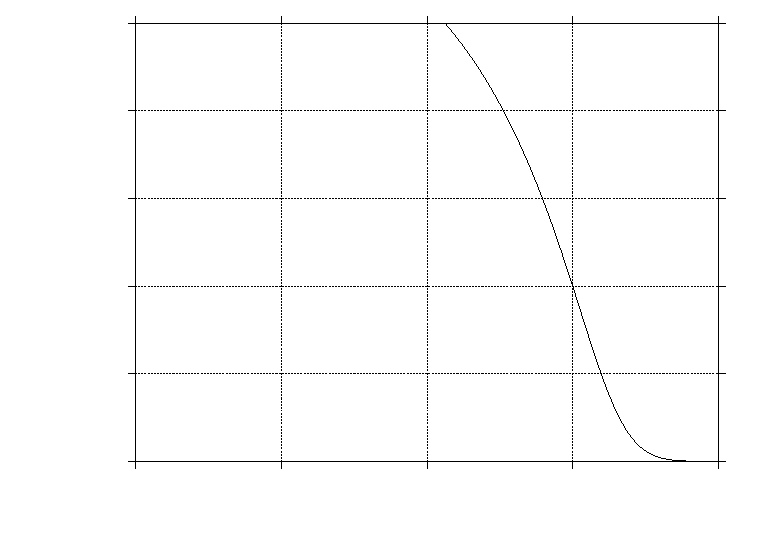
\includegraphics{Figures/twowires/Deltas4.5/Tdepend}}%
    \gplfronttext
  \end{picture}%
\endgroup
  
\caption{Blue solid line: $|\Delta^{12}_{k_F}|$ as a function of temperature. Blue dashed line: asymptotic form due to Landau's theory of phase transitions, equation \eqref{eq.DeltaasymptoteTc}. Red solid line: $|\Delta^{11}_{k_F}|$ as a function of temperature. Red dashed line: asymptotic form due to Landau's theory of phase transitions, equation \eqref{eq.DeltaasymptoteTc}. Notice, that there are two critical temperatures, and that the interwire pairing shows a downward kink, where the intrawire pairing goes to zero. \\
Parameters: $k_Fd = 0.759$, $(n_Ba_B^3)^{1/3} = 0.01$, $(n_Ba_{BF}^3)^{1/3} = 0.1$, $l_t = 0$, $m_B / m_F = 7/40$, $n_F / n_B^{1/3} = 0.215$, $v_F / c_0 = 0.33$.}  
\label{fig.maximalpairingsTdepend_2wires}  
\end{center}    
\end{figure}

The plot shows two phase transitions, one for each pairing. These happen at two different critical temperatures, $T^{11}_{c}$ and $T^{12}_{c}$. Near these phase transitions, it is a general result due to Landau, that the order parameter goes as $\sqrt{1 - T/T^{ij}_c}$, see section \ref{sec.landauphasetransitions} and \cite[86-87]{PlischkeStatPhys}. The pairing potentials are linearly dependent on the mean fields, $\braket{c_{i, -k}c_{j,k}}$, which are the order parameters in the present case. Hence, close to the critical temperatures $T^{ij}_c$ we must have:
\begin{equation}
\max_k[\Delta^{ij}_k](T) = \alpha_{ij} \max_k[\Delta^{ij}_k](T = 0) \sqrt{1 - T/T^{ij}_c}. 
\label{eq.DeltaasymptoteTc}
\end{equation}
We fit these functions to the data close to the critical temperatures by adjusting $\alpha_{ij}$. This results in the dashed lines in figure \ref{fig.maximalpairingsTdepend_2wires}, which fit near the critical temperatures as expected. 

In conclusion, the presence of a second type of pairing changes the functional dependency on temperature and lowers the dominant pairing. However, the calculated temperature dependency of the pairings are \textit{not} reliable. This is due to the increasing phase fluctuations with increasing temperature. Significant steps beyond our current formalism must be taken to come with more reliable calculations of the temperature dependency. 

